% Included from both -slides and -handout versions.

\mode<presentation>
{
  \usetheme{default}
  \useoutertheme{infolines}
}

\usepackage[english]{babel}
\usepackage[latin1]{inputenc}
\usepackage{graphicx}
\usepackage{times}
\usepackage[T1]{fontenc}
\usepackage{fancyvrb}
\usepackage{listings}
\begin{document}
\lstset{language=C, escapeinside={(*@}{@*)}, numbers=left,
  basicstyle=\tiny, showspaces=false, showtabs=false}

\title{L41: Advanced Operating Systems}
\subtitle{Through tracing, analysis, and experimentation}
%\institute{University of Cambridge}
%\author{George V. Neville-Neil}
\author{Dr Robert N. M. Watson}
\date{13 October 2015}

\begin{frame}
  \titlepage
\end{frame}

\section{Introduction}

\begin{frame}
  \frametitle{Getting started}

  \begin{enumerate}
    \item What is an operating system?
    \item Systems research
    \item About the module
    \item Lab reports
    \item Readings for next time
  \end{enumerate}
\end{frame}

\section{What is an operating system?}

%
% This interactive whiteboarding exercise should take five minutes or less:
% ask about places where OSes are used, what services they provide, what other
% problems can think of.  Where have OSes let them down?  What is in an OS?
%

\begin{frame}
  \begin{huge}
  \begin{center}
    What is an operating system?
  \end{center}
  \end{huge}

  \bigskip

  \begin{center}
  \begin{tiny}
    Whiteboarding exercise
  \end{tiny}
  \end{center}
\end{frame}

\begin{frame}
  \frametitle{What is an operating system?}

  \begin{large}
  \begin{center}
    [An OS is] low-level software that supports \\
    a computer's basic functions, such as \\
    scheduling tasks and controlling peripherals. \\
  \smallskip
  \small{- Google hive mind}
  \end{center}
  \end{large}
\end{frame}

\begin{frame}
  \frametitle{General-purpose operating systems}

  ...  are for general-purpose computers

  \begin{itemize}
    \item Servers, workstations, mobile devices
    \item Run `applications' -- i.e., software unknown at design time
    \item Abstract the hardware, provide `class libraries'
    \item E.g., Windows, Mac OS X, Android, iOS, Linux, FreeBSD, ...
  \end{itemize}

  \pause

  \medskip

  \begin{description}
    \item[\textbf{Userspace}]

      \smallskip

      Local and remote shells, management tools, daemons

      \smallskip

      Run-time linker, system libraries, tracing facilities

    \pause

    \item[] {\tiny - - - - \textit{system-call interface} - - - -}

    \pause

    \item[\textbf{Kernel}]

      System calls, hypercalls, remote procedure call (RPC)

      \smallskip

      Processes, filesystems, IPC, sockets, management

      \smallskip

      Drivers, packets/blocks, protocols, tracing, virtualisation

      \smallskip

      VM, malloc, linker, scheduler, threads, timers, tasks, locks

  \end{description}

  \pause

  \medskip

  Continuing disagreement on whether distributed-filesystem servers and
  window systems `belong' in userspace or the kernel
\end{frame}

\begin{frame}
  \frametitle{Other kinds of operating systems}

  \bigskip
  What if we specialise the OS for specific applications or environments?

  \pause
  \bigskip
  \begin{itemize}
    \item \textbf{Embedded operating systems}
    \begin{itemize}
      \item Serve a single application in a specific context
      \item Wireless access points, medical devices, washing machines, cars
      \item Small code footprint, real-time scheduling
      \item \textit{Might} have virtual memory / process model
      \item Microkernels or single-address space: VxWorks, RTEMS, L4
      \item Now also: Linux, BSD over a real-time kernel
    \end{itemize}

    \pause
    \bigskip

    \item \textbf{Appliance operating systems}
    \begin{itemize}
      \item Apply embedded model to higher-level devices/applications
      \item File storage appliances, routers, firewalls, ...
      \item E.g., Juniper JunOS, Cisco IOS, NetApp OnTap, EMC/Isilon
      \item Under the hood, almost always Linux, BSD, etc
    \end{itemize}
  \end{itemize}
\end{frame}

\begin{frame}
  \frametitle{Other kinds of operating systems (cont.)}

  \bigskip
  What if we rearrange the process-model and system-call boxes?

  \pause
  \bigskip

  \begin{itemize}
    \item \textbf{Microkernels, library operating systems, unikernels}
    \begin{itemize}
      \item Shift code out of the kernel into userspace to reduce TCB; \\
	improve robustness/flexibility; `bare-metal' apps
      \item Early 1990s: Microkernels are king!
      \item Late 1990s: Microkernels are too slow!
      \item 2000s/2010s: Microkernels are back! But now `hypervisors'
      \item Sometimes: alternative linkage (e.g., programming-language)
    \end{itemize}

    \pause
    \bigskip

    \item \textbf{Hypervisors}
    \begin{itemize}
      \item Kernels host applications; hypervisors host virtual machines
      \item Virtualised hardware interface rather than POSIX
      \item \textit{Paravirtualisation} reintroduces OS-like interfaces for
	performance
      \item A lot of microkernel ideas have found a home here
      \item E.g., System/370, VMware, Xen, KVM, VirtualBox, bhyve, ...
    \end{itemize}
  \end{itemize}
\end{frame}

\begin{frame}
  \frametitle{What does an operating system do?}

  \begin{itemize}
    \item Key hardware-software surface (cf. compilers)
    \item System management: bootstrap, shutdown, watchdogs
    \item Low-level abstractions and services
    \begin{itemize}
      \item Programming: processes, threads, IPC, program model
      \item Resource sharing: scheduling, multiplexing, virtualisation
      \item I/O: device drivers, local/distributed filesystems, network stack
      \item Security: authentication, encryption, permissions, labels, audit
      \item Local or remote access: console, window system, SSH
    \end{itemize}
    \item Libraries: math, protocols, RPC, cryptography, UI, multimedia
    \item Other stuff: system log, debugging, profiling, tracing
  \end{itemize}

  \pause
  \bigskip

  Compiler?  Text editor?  E-mail package?  Web browser?  Can an operating
  system be `distributed'?
\end{frame}

\section{Why study operating systems?}

\begin{frame}
  \frametitle{Why study operating systems?}

  \bigskip

  The OS plays a central role in \textbf{whole-system design}  when building
  efficient, effective, and secure systems:

  \bigskip

  \begin{itemize}
    \item Key interface between hardware and software
    \item Strong influence on whole-system performance
    \item Critical foundation for computer security
    \item Exciting programming techniques, algorithms, problems
    \begin{itemize}
      \item Virtual memory; network stacks; filesystems; runtime linkers; ...
    \end{itemize}
    \item Co-evolves with platforms, applications, users
    \item Multiple active research communities
    \item Reusable techniques for building complex systems
    \item Boatloads of fun (best text adventure ever)
  \end{itemize}
\end{frame}

\begin{frame}
  \frametitle{Where is the OS research?}

  \bigskip
  A sub-genre of \textit{systems research}:
  \bigskip

  \begin{itemize}
    \item Evolving hardware-software interfaces
    \begin{itemize}
      \item New computation models / architectures
      \item New kinds of peripheral devices
    \end{itemize}
    \item Integration with programming languages and runtimes
    \item Concurrent/parallel programming models; scheduling
    \item Security and virtualisation
    \item Networking, storage, and distributed systems
    \item Tracing and debugging techniques
    \item As a platform for other research -- e.g., mobile systems
  \end{itemize}

  \pause
  \bigskip
  Venues: SOSP; OSDI; USENIX ATC; EuroSys; HotOS; FAST; NSDI; HotNets;
  ASPLOS; USENIX Security; ACM CCS; IEEE S\&P; ...
\end{frame}

\begin{frame}
  \frametitle{What are the research questions?}

  Just a few examples: by changing the OS, can I...
  \bigskip

  \begin{itemize}
    \item create new abstractions for new hardware?
    \item make my application run faster by...
    \begin{itemize}
      \item better masking latency?
      \item using parallelism more effectively?
      \item exploiting new storage mediums?
      \item adopting distributed-system ideas in local systems?
    \end{itemize}
    \item make my application more \{reliable, power efficient\}
    \item limit the \{security, privacy\} implications of bad/exploited
      programs?
    \item use new languages/analysis techniques in new ways?
  \end{itemize}

  \pause
  \bigskip
  Systems research focuses on \textbf{evaluation} with respect to
  \textbf{applications} or \textbf{workloads}: how can we measure whether it
  is \{faster, better, ...\}?
\end{frame}

\section{About L41}

\begin{frame}
  \frametitle{Teaching operating systems}

  \begin{itemize}
    \item Two common teaching tropes:
    \begin{itemize}
      \item \textbf{Trial by fire}: in micro, recreate classic elements of
	operating systems: microkernels with processes, filesystems, etc
      \item \textbf{Research readings course}: read, present, discuss, and
	write about classic works of systems research
    \end{itemize}

    \pause
    \bigskip

    \item This module adopts elements of both approaches while:
    \begin{itemize}
      \item mitigating the risk of OS kernel hacking in a short course;
      \item working on real-world systems rather than toys; and
      \item targeting research skills not just operating-system design
    \end{itemize}

    \pause
    \bigskip

    \item Trace and analyse real systems driven by synthetic benchmarks
    \item Possible only because of recent developments in tracing

  \end{itemize}
\end{frame}

\begin{frame}
  \frametitle{Aims of the module}

  Teach methodology, skills, and knowledge required to understand and perform
  research on contemporary operating systems by...

  \begin{itemize}
    \item Teaching systems-analysis methodology and practice
    \item Exploring real-world systems artefacts
    \item Developing scientific writing skills
    \item Reading selected original systems research papers
  \end{itemize}
\end{frame}

\begin{frame}
  \frametitle{Prerequisites}

  We will take for granted:
  \bigskip

  \begin{itemize}
    \item High-level knowledge of operating systems gained in an undergraduate
      course (or equivalent); e.g.:
    \begin{itemize}
      \item What schedulers do
      \item What processes are... and how they differ from threads
      \item What Interprocess Communication (IPC) does
      \item How a simple filesystem might work
    \end{itemize}
    \item Reasonable fluency in reading/producing multithreaded C
%    \item Modest Python skills
    \item Comfort with the UNIX command-line environment
    \item Undergraduate skills with statistics \\
      {\tiny (mean/median/mode/stddev/\textit{t}-tests/linear regression/boxplots/scatterplots/...)}
  \end{itemize}

  \pause
  \bigskip
  You can pick up some of this as you go (e.g., IPC, \textit{t}-tests), but
  will struggle if you are missing most of these
\end{frame}

\begin{frame}
  \frametitle{Module structure}

  \begin{itemize}
    \item {\bf One-hour lectures} in FS-07 ($\times$6)
    \begin{itemize}
      \item Theory, methodology, architecture, and practice
    \end{itemize}

    \pause
    \bigskip
    \item {\bf Two-hour labs} in SW-02 ($\times$5)
    \begin{itemize}
      \item 10--20-minute lecturelets on artefacts and practical skills
      \item Remainder on hands-on measurement and experimentation
      \item Optional \textit{exploratory questions} vs. \textit{experimental
	goals}
    \end{itemize}

    \pause
    \bigskip
    \item {\bf Assigned readings}
    \begin{itemize}
      \item Selected portions of module texts
      \item Historic and contemporary research papers
    \end{itemize}

    \pause
    \bigskip
    \item {\bf Assessed lab reports}
    \begin{itemize}
      \item Based on experiments done in (and out) of labs
      \item Refine scientific writing style suitable for systems research
      \item One `practice run' marked but not assessed
      \item Two assessed; 50\% of final mark each
    \end{itemize}
  \end{itemize}
\end{frame}

\begin{frame}
  \frametitle{Rough module schedule and decomposition}

  \begin{itemize}
    \item Submodule 1: Introduction to kernels and tracing/analysis
    \begin{itemize}
      \item 2 lectures, 1 lab (I/O)
      \item Introduction: OSes, Systems Research, and L41
      \item The Kernel: Kernel and Tracing
      \item First lab report due
    \end{itemize}

    \pause
    \bigskip
    \item Submodule 2: The Process Model
    \begin{itemize}
      \item 2 lectures, 2 labs (IPC, PMC)
      \item The Process Model (1) - Binaries and Processes
      \item The Process Model (2) - Traps, System Calls, and Virtual Memory
      \item Second lab report due
    \end{itemize}

    \pause
    \bigskip
    \item Submodule 3: TCP/IP
    \begin{itemize}
      \item 2 lectures, 2 labs (TCP state machine, congestion control)
      \item The Network Stack (1) - Sockets, NICs, and Work Distribution
      \item The Network Stack (2) - TCP protocol
      \item Final lab report due
    \end{itemize}
  \end{itemize}
\end{frame}

\begin{frame}
  \frametitle{The platform}

  \begin{itemize}
    \begin{columns}[T]
    \column{0.4\textwidth}

      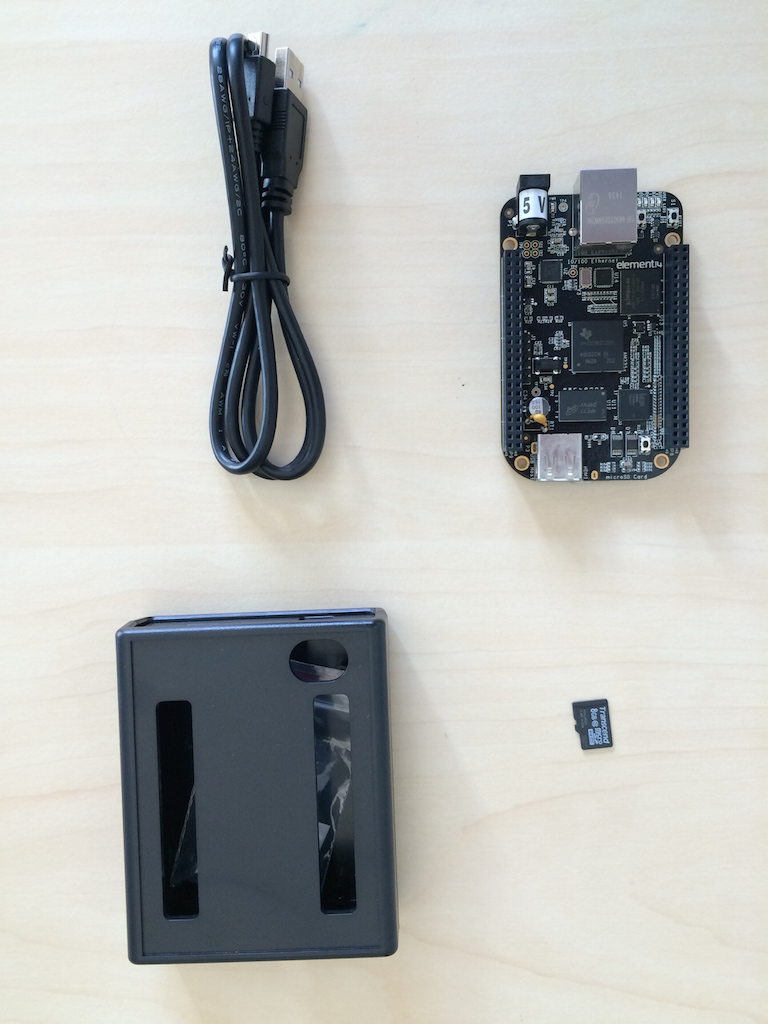
\includegraphics[width=\textwidth,keepaspectratio]{../../figures/bbb-onna-desk.jpg}

    \column{0.4\textwidth}
      \item BeagleBone Black
      \item 1GHz ARM Cortex A-8 32-bit CPU
      \item Superscalar pipeline, MMU, L1/L2 caches
      \item FreeBSD operating system
      \item DTrace
      \item `potted benchmarks'
    \end{columns}
  \end{itemize}
\end{frame}

\begin{frame}
  \frametitle{Labs and lab reports}

  Lab reports document an experiment and analyse its results -- typically in
  the context of a hypothesis that will be tested.
  \medskip

  A lab report will contain at least the following sections:

  \begin{enumerate}
    \begin{columns}[T]
    \column{0.4\textwidth}
      \item Title + abstract
      \item Introduction
      \item Experimental setup and methodology
    \column{0.4\textwidth}
      \item Results and discussion
      \item Conclusion
      \item References
      \item Appendices
    \end{columns}
  \end{enumerate}

  Some formats break out sections experimental setup vs.  methodology, and
  results vs. discussion.  The combined format seems to work better for
  systems experimentation as compared to, say, biology.
  \medskip

  See lab-report notes on the website.
\end{frame}

\begin{frame}
  \frametitle{Module texts - core material}

  You will need to make frequent reference to these books both in the labs and
  outside of the classroom:

  \begin{itemize}
    \item {\bf Operating systems}: Marshall Kirk McKusick, George V.
      Neville-Neil, and Robert N. M. Watson, \textit{The Design and
      Implementation of the FreeBSD Operating System, 2nd Edition}, Pearson
      Education, Boston, MA, USA, September 2014.

    \pause
    \bigskip
    \item {\bf Performance measurement}: Raj Jain, \textit{The Art of Computer
      Systems Performance Analysis: Techniques for Experimental Design,
      Measurement, Simulation, and Modeling}, Wiley - Interscience, New York,
      NY, USA, April 1991.

    \pause
    \bigskip
    \item {\bf Tracing and profiling}: Brendan Gregg and Jim Mauro,
      \textit{DTrace: Dynamic Tracing in Oracle Solaris, Mac OS X and
      FreeBSD}, Prentice Hall Press, Upper Saddle River, NJ, USA, April 2011.
  \end{itemize}
\end{frame}

\begin{frame}
  \frametitle{Module texts - supplemental material}

  If your OS recollections feel a bit hazy:

  \begin{itemize}
    \item {\bf Operating systems}: Abraham Silberschatz, Peter Baer Galvin,
      and Greg Gagne, \textit{Operating System Concepts, Eighth Edition}, John
      Wiley \& Sons, Inc., New York, NY, USA, July 2008.
  \end{itemize}

  \pause
  \bigskip
  If you want to learn a bit more about architecture and measurement:

  \begin{itemize}
    \item {\bf Performance measurement and diagnosis}: Brendan Gregg,
      \textit{Systems Performance: Enterprise and the Cloud}, Prentice Hall
      Press, Upper Saddle River, NJ, USA, October 2013.
  \end{itemize}
\end{frame}

%\begin{frame}
%  \frametitle{Lectures and lecturelets}
%
%  \begin{enumerate}
%    \item Introduction: OSes, systems research, the module
%    \item Kernel design overview
%    \item The process model (1)
%    \item The process model (2)
%    \item The network stack (1)
%    \item The network stack (2)
%  \end{enumerate}
%
%  \begin{enumerate}
%    \item Getting started with DTrace
%    \item Getting a bit further with DTrace
%    \item Getting started with PMC
%    \item Tracing the TCP state machine
%    \item Tracing TCP congestion control
%  \end{enumerate}
%\end{frame}

%\begin{frame}
%  \frametitle{Suggested papers}
%
%  \begin{itemize}
%   \item \cite{Cantrill:2007cw}
%   \item \cite{Anderson:1992wh}
%   \item \cite{Marinos:2014hr}
%   \item \cite{Ridge:2008uo}
%   \item \cite{Saltzer:1984wi}
%   \item \cite{McCanne:1993vga}
%  \end{itemize}  
%\end{frame}

\begin{frame}
  \frametitle{Reading for Next Lecture}

  \begin{itemize}
    \item McKusick, et al. - Chapter 3
    \item Cantrill, et al. 2004 - full article
  \end{itemize}
\end{frame}

\end{document}
